\specialchapter{Invariances under completion}

\begin{enumerate}
\def\labelenumi{(\alph{enumi})}
\tightlist
\item
  Let A be a ring and m an ideal of A distinct from A. Let A be given the m-adic topology and let \(\hat{A}\) denote its Hausdorff completion.
\end{enumerate}

A Hausdorff

YES

A Noetherian

YES (III, § 3, Proposition 8)

A local

YES (III, § 2, Proposition 19)

A semi-local

YES (III, § 2, Corollary to Proposition 19)

A a Zariski ring

YES (III, § 3, Proposition 8)

\textbf{\(\hat{\mathbf{A}}\)}\par

\begin{enumerate}
\def\labelenumi{(\alph{enumi})}
\setcounter{enumi}{1}
\tightlist
\item
  Suppose now that \(\mathbf{A}\) is local and Noetherian and that \(\mathfrak{m}\) is its maximal ideal.
\end{enumerate}

A an integral domain

A an integrally closed domain

A a discrete valuation ring

A reduced

\textbf{\(\hat{\mathbf{A}}\)}\par

NO (III, § 3, Exercise 15 (b))

YES for excellent rings (1)

%\pandocbounded{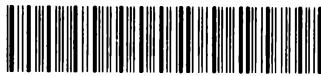
\includegraphics[keepaspectratio]{images/part004_82ba3e9c.jpg}}\\

